\documentclass[11pt]{article}

\usepackage[margin=2cm, a4paper]{geometry}	%2cm page margin
\usepackage{fancyhdr}						%use fancy headers
\usepackage{graphicx}						%use images
\usepackage{textcomp}						%used for textdegree command
\usepackage[hidelinks]{hyperref}            %used for clickable references
\usepackage{draftwatermark}
\SetWatermarkLightness{ 0.9 }
\SetWatermarkText{Preliminary}
\SetWatermarkScale{ 4 }

%DPTECHNICS datasheet variables
\newcommand{\dptproduct}{Walter - WiFi/BLE/NB-IoT/LTE-M module}

%page footers and headers settings
\pagestyle{fancy}
\fancyhead{}
\fancyfoot{}
\fancyhead[LO,LE]{ {\bf \dptproduct}}
\fancyfoot[R]{\thepage}
\fancyfoot[L]{QuickSpot - 2023}
\renewcommand{\footrulewidth}{0.4pt}
\renewcommand\familydefault{\sfdefault}
\setlength{\parindent}{0pt}

\begin{document}
\begin{titlepage}
\hfill
\includegraphics[width=8cm]{logo.pdf}\\

\hfill {\bf \Large  \dptproduct}\\[-3mm]

\hfill {\Large Preliminary Datasheet}

\vfill
\rule{487pt}{1pt}

\hfill Revision 0.2 - \today
\end{titlepage}
\section{General information}
Walter is an ESP32-S3 based IoT board that offers WiFi, Bluetooth 5 (LE), cellular CAT M1/NB1/NB2 and GNSS connectivity. 

\section{Features}
Walter is based on an ESP32-S3-WROOM-1-N16R2 module with an on-board Sequans GM02SP modem.
This combination makes Walter a unique development board that offers a rich feature-set which include but is not limited to:
\begin{itemize}
	\item CPU: Xtensa Dual-core 32-bit LX7 CPU (ESP32-S3 SoC)
	\item RAM: 2MB (Quad SPI) PSRAM
	\item Flash: 16MB (Quad SPI) Flash memory
	\item WiFi: 150Mbps(n) 802.11 WiFi b/g/n with on-board antenna
	\item LTE: CAT M1/NB1/NB2 (GM02SP module)
	\item GPS: GPS, GNSS Constellation support (GM02SP module)
	\item Bluetooth: 2Mbps Bluetooth 5 (LE), Bluetooth Mesh
	\item 24 physical GPIO pins 
\end{itemize}
\section{Absolute maximum ratings}
For the most reliable use and stability of the module we advice to use the typical ratings. We do not guarantee the correct functioning of the device outsite the minimum and maxium range of the module. 
\begin{center}
\renewcommand{\arraystretch}{1.5}
\begin{tabular}{|p{5cm}|c|c|c|c|}
\hline
{\bf Parameter} & {\bf Units} & {\bf Minimum rating} & {\bf Typical rating} & {\bf Maxium rating} \\
\hline
\hline
DC Supply Voltage & V & 3.0 & 5.0 & 5.5 \\
\hline
Digital I/O Voltage & V & 2.64 & 3.3 & 3.6 \\
\hline
\end{tabular}
\end{center}

\newpage
\section{Interfaces}
Walter provides a total of 28 physical pins (3 power, 1 strapping and 24 IO) to interface with external parts. This chapter provides information about these pins as well as internally connected pins and the testpoints located at the bottom of the board.\newline

Power supply pins and their details are available in section \ref{power} about the power characteristics.\newline

For more information about specific pins regarding the ESP32-S3 Wroom module or the Sequans GM02SP module, please refer to the datasheet of the corresponding module.

\subsection{Pin Assignment} \label{pin_assigment}

\begin{figure}[h]
    \centering
    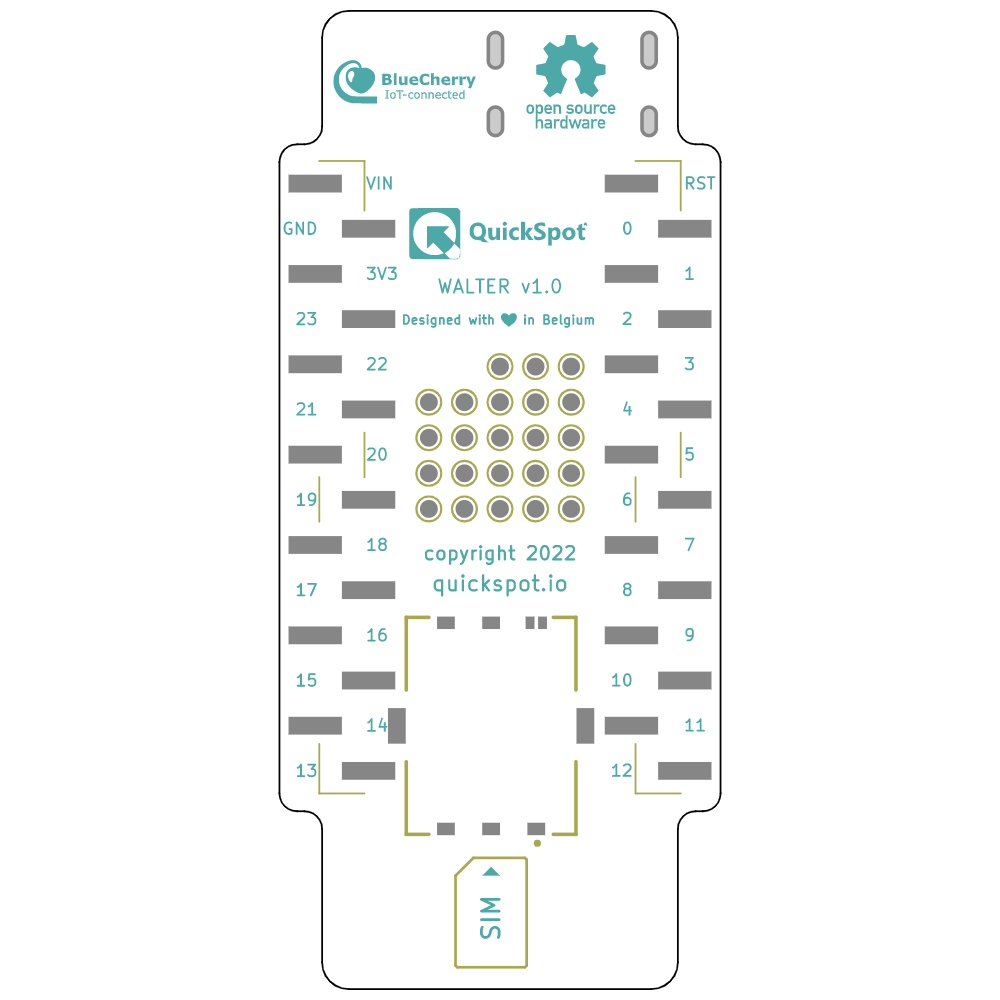
\includegraphics[height=11cm]{back_pinout.png}
    \caption{Walter Board Pin Assigment}
    \label{fig:walter_pin_assignment}
\end{figure}
\newpage
\subsubsection{External Pins} \label{external_pins}
Table \ref{table_exteral_pin} contains the description of the physical pins on Walter available on the underside of the board. \newline
The order of this table, in reference to the board, is top to bottom and left to right.\newline
\renewcommand{\arraystretch}{1.5}
\begin{table}[!h]
\begin{center}
\begin{tabular}{|c|c|c|c|p{9.5cm}|}
\hline
{\bf Pin} & \multicolumn{1}{c|}{\bf ESP pin} & \multicolumn{1}{c|}{\bf Input/Output} & \multicolumn{1}{c|}{\bf Description} \\
\hline
\hline
VIN & N/A & power input & DC Power Input (Characteristics \ref{power})\\
\hline
GND & N/A & power input & GND Connection \\
\hline
3V3 SWITCHED & N/A & power output & Switchable +3.3VDC output (Characteristics \ref{power}) \\
\hline
10 & IO10 & bidirectional & General purpose I/O \\
\hline
9 & IO9 & bidirectional & General purpose I/O \\
\hline
8 & IO8 & bidirectional & General purpose I/O \\
\hline
18 & IO18 & bidirectional & General purpose I/O \\
\hline
17 & IO17 & bidirectional & General purpose I/O \\
\hline
16 & IO16 & bidirectional & General purpose I/O \\
\hline
15 & IO15 & bidirectional & General purpose I/O \\
\hline
7 & IO7 & bidirectional & General purpose I/O \\
\hline
6 & IO6 & bidirectional & General purpose I/O \\
\hline
5 & IO5 & bidirectional & General purpose I/O \\
\hline
4 & IO4 & bidirectional & General purpose I/O \\
\hline
EN & RESET & input & ESP32 reset with 10k pullup \\
\hline
RX0 & RXD0 & bidirectional & ESP32 UART0 Receive \\
\hline
TX0 & TXD0 & bidirectional & ESP32 UART0 Transmit \\
\hline
0/3V3\_EN & IO0 & bidirectional & Bootloader and 3.3VDC switch after boot \\
\hline
12 & IO12 & bidirectional & General purpose I/O \\
\hline
11 & IO11 & bidirectional & General purpose I/O \\
\hline
13 & IO13 & bidirectional & General purpose I/O \\
\hline
38 & IO38 & bidirectional & General purpose I/O \\
\hline
39 & IO39 & bidirectional & General purpose I/O \\
\hline
40 & IO40 & bidirectional & General purpose I/O \\
\hline
41 & IO41 & bidirectional & General purpose I/O \\
\hline
42 & IO42 & bidirectional & General purpose I/O \\
\hline
2 & IO2 & bidirectional & General purpose I/O \\
\hline
1 & IO1 & bidirectional & General purpose I/O \\
\hline
\end{tabular}
\caption{\label{table_exteral_pin}Walter External Pin Definitions}
\end{center}
\end{table}
\newpage

\subsubsection{Internal Pins} \label{internal_pins}
Table \ref{table_interal_pin} contains the pin descriptions of the internally connected GPIO pins on Walter. These are necessary for either communication between components on the board or reserved for other purposes and thus not available for external use.

\begin{table}[!h]
    \centering
    \begin{tabular}{|c|p{9.5cm}|}
    \hline
    {\bf ESP pin} & \multicolumn{1}{c|}{\bf Description} \\
    \hline
    \hline
    IO19 & USB D-\\
    \hline
    IO20 & USB D+\\
    \hline
    IO46 & LTE\_WAKE0 \\
    \hline
    IO45 & LTE\_UART0\_TX (See \ref{lte_uart})\\
    \hline
    IO14 & LTE\_UART0\_RX (See \ref{lte_uart})\\
    \hline
    IO21 & LTE\_UART0\_RTS (See \ref{lte_uart})\\
    \hline
    IO47 & LTE\_UART0\_CTS (See \ref{lte_uart})\\
    \hline
    IO48 & LTE\_RESET\\
    \hline
    \end{tabular}
    \caption{\label{table_interal_pin}Walter Internal Pin Definitions}
\end{table}
\newpage
\subsubsection{Testpoints} \label{testpoints}
Walter contains 23 testpoints on the bottom of the board that serve multiple purposes. You can use these pins for debugging, interfacing and/or flashing of the Sequans GM02SP and the ESP32-S3-WROOM Modules.
\begin{figure}[h]
    \centering
    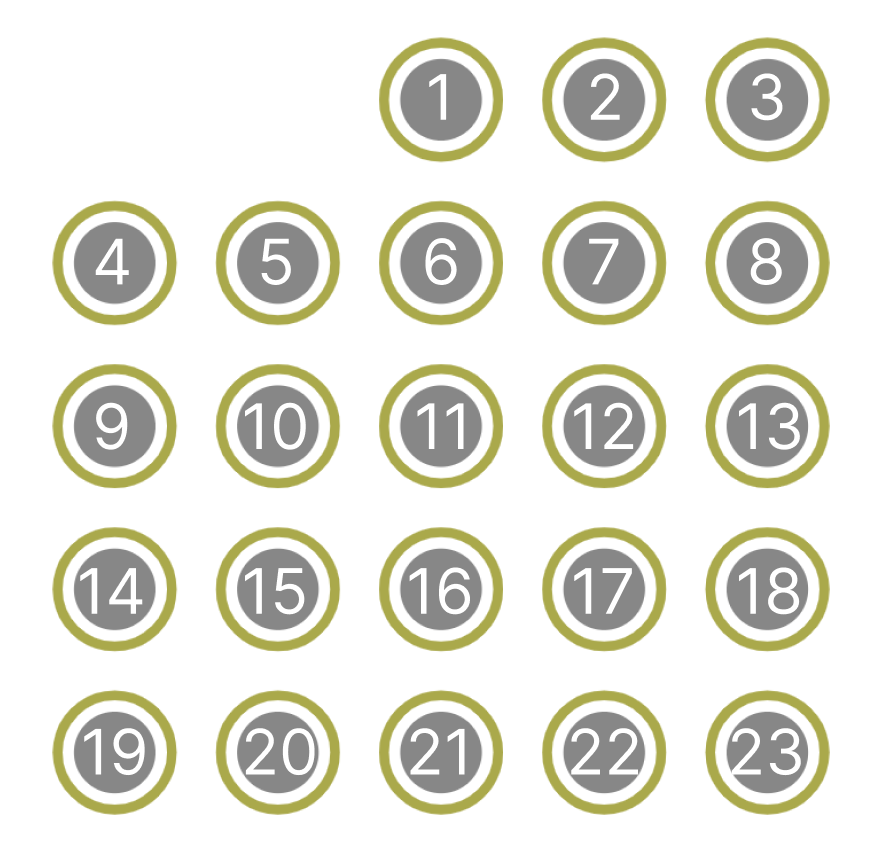
\includegraphics[height=5cm]{testpoints.png}
    \caption{Walter Testpoints Layout}
    \label{fig:testpoints}
\end{figure}

Table \ref{tab:testpoints} contains the description of the testpoints as depicted in Figure \ref{fig:testpoints}.
\begin{center}
\begin{tabular}{|c|p{9.5cm}|}
    \hline
    {\bf Number} & \multicolumn{1}{c|}{\bf Description} \\
    \hline
    \hline
    1 & LTE\_JTAG\_TRSTN\\
    \hline
    2 & LTE\_JTAG\_TCK\\
    \hline
    3 & LTE\_JTAG\_TDO\\
    \hline
    4 & LTE\_UART2\_RTS\\
    \hline
    5 & LTE\_UART2\_CTS\\
    \hline
    6 & LTE\_PS\_STATUS\\
    \hline
    7 & LTE\_JTAG\_TDI\\
    \hline
    8 & LTE\_JTAG\_TMS\\
    \hline
    9 & LTE\_UART2\_RX\\
    \hline
    10 & LTE\_UART1\_RX\\
    \hline
    11 & LTE\_UART1\_TX\\
    \hline
    12 & LTE\_UART0\_TX (Connected to ESP32 GPIO45)\\
    \hline
    13 & LTE\_UART0\_RX (Connected to ESP32 GPIO14)\\
    \hline
    14 & LTE\_UART2\_TX\\
    \hline
    15 & LTE\_UART1\_RTS (Pull-up R4 not fitted)\\
    \hline
    16 & LTE\_UART1\_CTS (Pull-up R6 not fitted)\\
    \hline
    17 & LTE\_UART0\_RTS (100k pull-up)\\
    \hline
    18 & LTE\_UART0\_CTS (100k pull-up)\\
    \hline
\end{tabular}
\end{center}
\newpage
\begin{table}[!h]
    \centering
    \begin{tabular}{|c|p{9.5cm}|}
    \hline
    {\bf Number} & \multicolumn{1}{c|}{\bf Description} \\
    \hline
    \hline
    19 & ESP\_GPIO3 (Strapping pin)\\
    \hline
    20 & GND\\
    \hline
    21 & +1.8VDC REF from GM02SP\\
    \hline
    22 & +3.3VDC\\
    \hline
    23 & VBUS\\
    \hline
    \end{tabular}
    \caption{Walter Testpoints Description}
    \label{tab:testpoints}
\end{table}

\subsubsection{Others}
Not all pins of the ESP32-S3 and Sequans GM02SP on Walter are internally connected, available through physical pins or testpoints. These pins are either reserved for use by the component itself or deemed not necessary to be available externally.

\subsection{LTE UART} \label{lte_uart}
The Sequans GM02SP module has 3 UART interfaces available by default. Only UART0 is connected to the ESP32-S3 Wroom Module on Walter as shown in Table \ref{table_interal_pin}. Communication between modules is possible with AT-commands. Please refer to the corresponding AT Command reference manual of the Sequans GM02SP for all possible AT-commands.


\section{Electrical and RF Characteristics} \label{power_rf_characteristics}
\subsection{Power} \label{power}
\subsubsection{Power Input}
Walter can be powered either by connecting a USB-C cable (see USB\_SECTION\_HERE) or via the VIN pin (see pinout \ref{external_pins}).\newline

\textbf{DO NOT} power Walter with both the USB-C connection and the VIN-pin! This can lead to seriously damaging the board and external peripherals connected to it!
\subsubsection{Power Output}
Walter contains a Texas Instruments LM3281YFQR DC-DC Converter which takes power from either the USB-C port or the VIN-pin and converts it to a regulated +3.3VDC supply.
\subsubsection{Power Consumption}
\subsection{GPIO} \label{gpio}
All GPIO pins exposed via the physical pin headers on Walter are 3.3V resistant. If you want to connect 5V or other forms of logic, please use a suitable logic level converter or voltage divider.\newline

Please reference the corresponding datasheets for all minimum, maximum and typical ratings of I/O pins of the ESP32-S3-WROOM or Sequans GM02SP Modules that may or may not be exposed on the Walter Development Board.
\subsection{RF}
\newpage
\section{Mechanical information}
\begin{figure}[h]
    \centering
    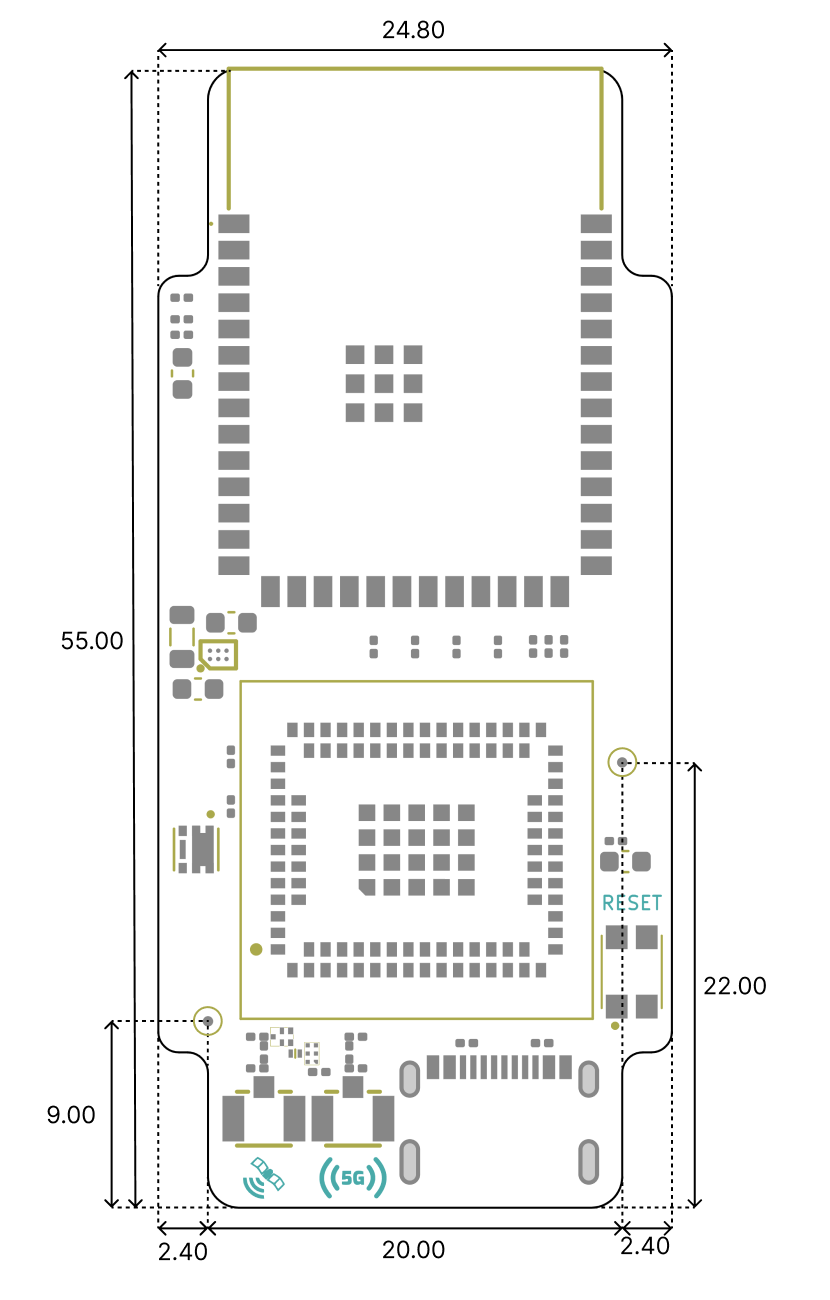
\includegraphics[height=13cm]{mechanical-front.png}
    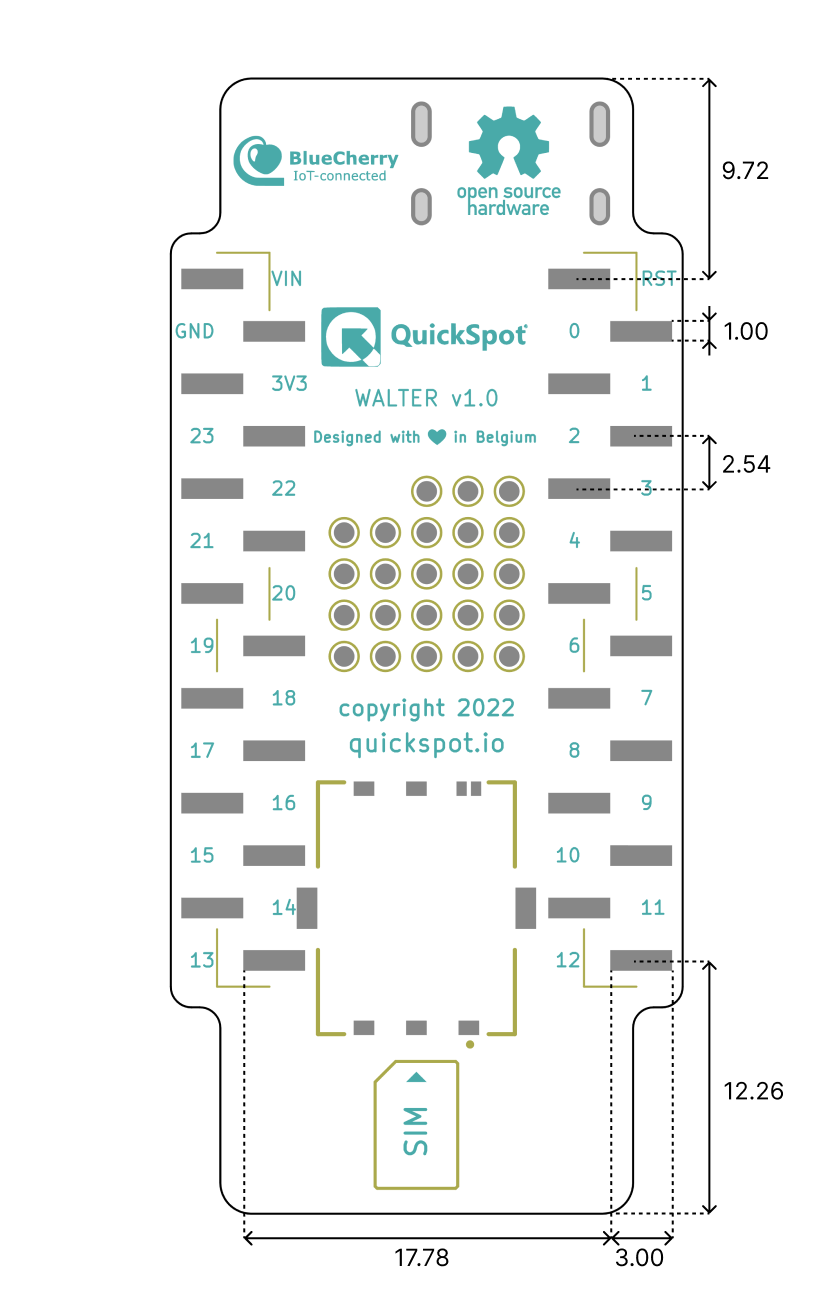
\includegraphics[height=13cm]{mechanical-back.png}
    \caption{Mechanical Drawing Front and Rear View - Unit in mm}
    \label{fig:mechanical_front}
\end{figure}

\section{Software}
Walter comes without firmware out of the box. You can easily program and upload your own firmware for Walter using MicroPython, Arduino, ESP-IDF... 
Please refer to the "Getting Started with Walter" available on our GitHub to get you up and running fast.

\section{Operating conditions}
The module can operate in a wide range of temperatures and conditions. The following are guidelines in which the module is guaranteed to work correctly. 
\begin{center}
\renewcommand{\arraystretch}{1.5}
\begin{tabular}{|p{5cm}|c|c|c|c|}
\hline
{\bf Parameter} & {\bf Units} & {\bf Minimum rating} & {\bf Typical rating} & {\bf Maxium rating} \\
\hline
\hline
Working temperature & \textdegree C & -40 &  & 85 \\
\hline
Storage temperature & \textdegree C & -40 &  & 100 \\
\hline
Humidity & \%RH & 10 &  & 90 \\
\hline
Storage humidity & \%RH & 5 & & 90 \\
\hline
\end{tabular}
\end{center}
Please note that no condensation may occur on the PCB and components. 


\section{Legal information}
This module is distributed worldwide by DPTechnics bv. We are not responsible for any product this module is part of. This datasheet is made with great care for detail but it can be possible the datasheet will be updated with more accurate data in te future. Users of DPTechnics bv products can contact us by letter, telephone or email. \\

\noindent DPTechnics bv\\
Westkapellestraat 396/44\\
8300 Knokke-Heist\\
Belgium\\

\noindent Tel: +32(0)50 62 13 79\\
email: info@quickspot.io\\
web: https://www.quickspot.io
\end{document}
